\newpage
\section{Non-Cooperative Conflict Resolution}\label{sec:nonCooperativeConflictResolution}

\paragraph{Idea:} There is \emph{main UAS(1)} which is flying in open \emph{non-controlled} airspace. Other UAS are operating in its vicinity. It is expected that they are claiming their \emph{planned trajectories}. The \emph{Main UAS(1)} detects the collision with other \emph{UAS}(2-4).

There is no \emph{final decision maker} nor \emph{supervising authority}; all communication participants have a similar level of rights. 
\begin{note}
    There is an assumption that other airspace users are behaving like intruders, without intent to destroy or harm. The \emph{adversarial behavior} is not accounted. The response from an \emph{intruder} is not mandatory in \emph{non-controlled} airspace.
\end{note}

\paragraph{Goal:} Provide \emph{mutual avoidance mechanism} in \emph{non-controlled} airspace. Let us consider the equal standpoint of all airspace attendants.

\paragraph{Conflict Resolution:} The conflict resolution depends on current mode and \emph{handshake} between airspace attendants. The non-cooperative behavior has been implemented as follows:

\begin{enumerate}
    \item\emph{Navigation mode} - every \emph{airspace attendant} is calculating own \emph{collision cases} and checking the behavior of the other (virtual UTM).
    
    \item\emph{Emergency avoidance mode} - is depending on communication mode:
    \begin{enumerate}[a]
        \item\emph{Response mode} - claiming separation methods and using avoidance mechanism (Avoidance grid with intruder model in our case).
        
        \item\emph{Blind mode} - every conflict side picks own strategy respecting given \emph{rules of the air}.
    \end{enumerate}
\end{enumerate}

\begin{note}
    \emph{Intruder Intersection model selection:} UAS based on Event detects possible collision for some reason UTM directive is out of the question, then try to claim separation (body volume intruder model (app. \ref{s:bodyvolumeIntersection})), If separation fails, go full survival mode (uncertain intruder model (app. \ref{s:bodyvolumeIntersection})).
\end{note}

\paragraph{Special Cases in Manned Aviation:} There are IFALPA reports which can give us an overview of \emph{enforced non-cooperative} mode causes in \emph{controlled airspace}:  
\begin{enumerate}
    \item \emph{VFR disabled} - flying in fog or thick clouds can render pilot vision, similar to UAS cameras/LiDAR.
    
    \item \emph{IFR equipment broke} - the sensor malfunction is more likely to happen due to the lesser redundancy in UAS systems.
    
    \item \emph{C2C Link disabled} - communication loss is more likely to happen, due to the lesser redundancy.
    
    \item \emph{ATM failure} - the ground control module of UTM can also fail.
\end{enumerate}

\begin{note}
    Traffic management related fails are lesser than 0.001 cases per one flight (according to IFALPA \cite{subotic2007recovery}).
\end{note}

\begin{figure}[H]
    \centering
    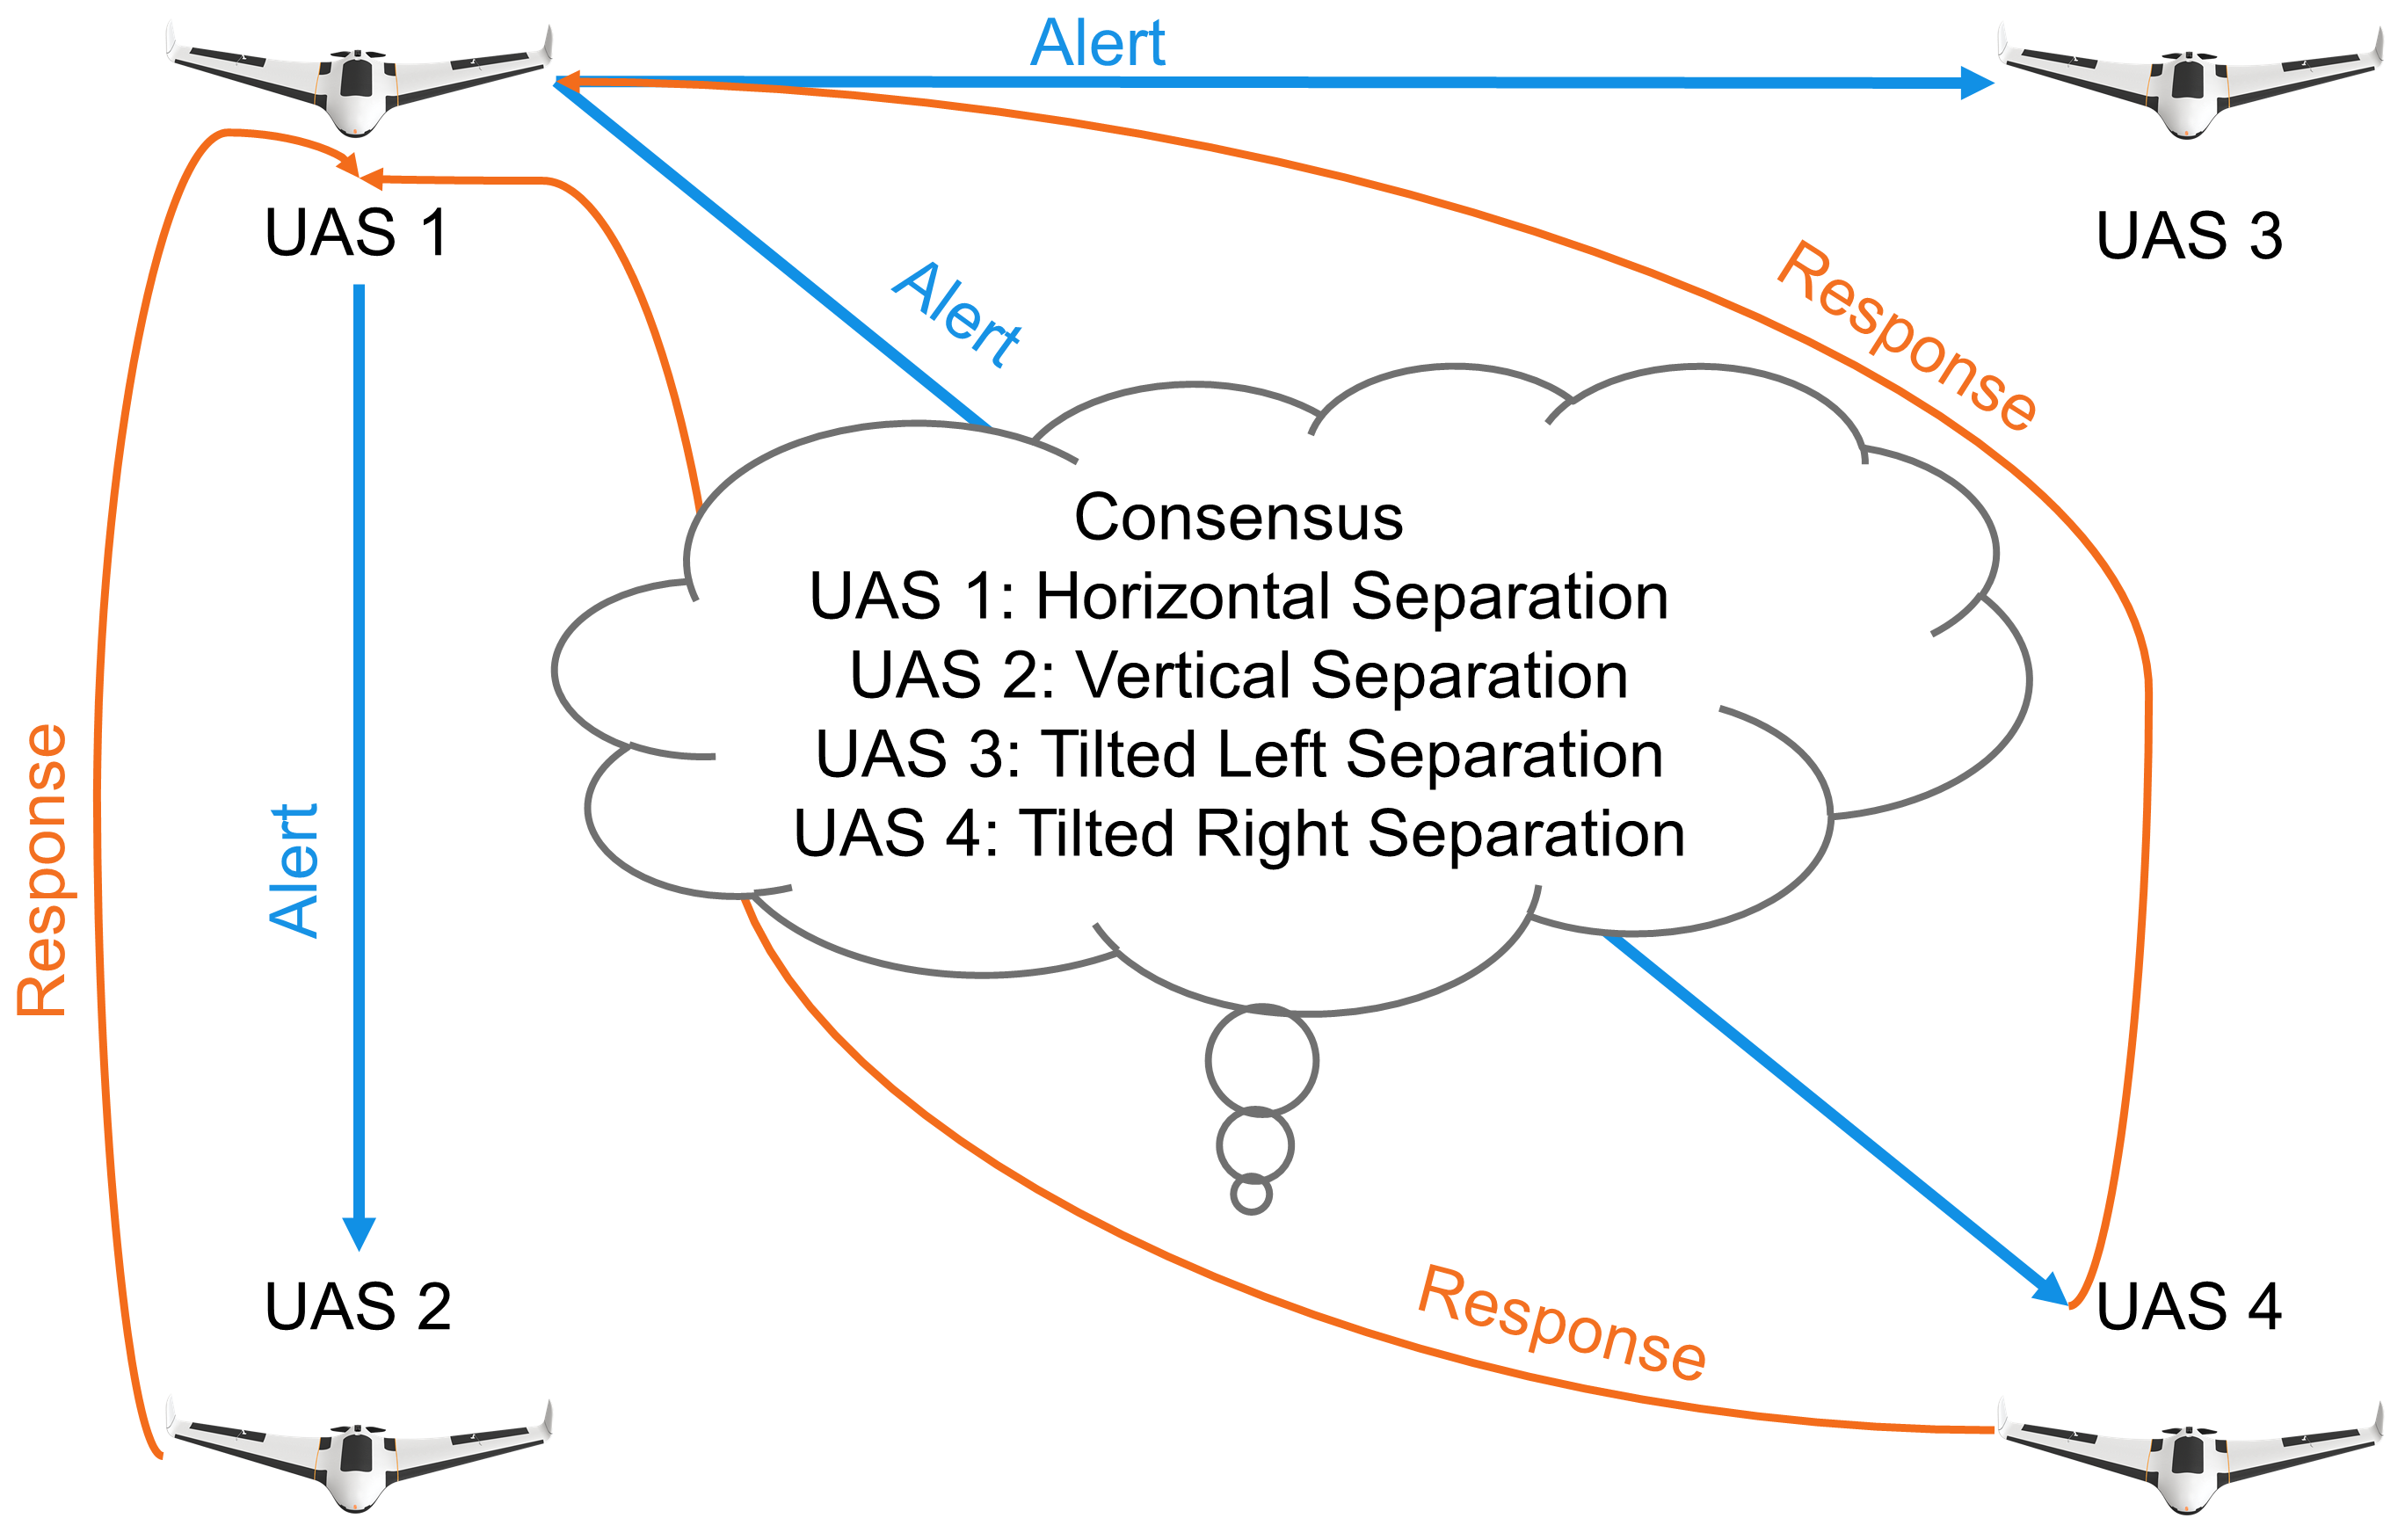
\includegraphics[width=0.7\linewidth]{\FIGDIR/RE004NonCooperativeResolution} 
    \caption{Non-cooperative conflict resolution via UAS claims.}
    \label{fig:NonCooperativeConflictResolutionUTM}
\end{figure}

\paragraph{Response mode scenario example:} The \emph{main UAS(1)} is going to collide with other \emph{UAS}(2-4):
\begin{enumerate}
    \item $UAS(1) \to UAS(2-4)$ sends position and heading notification.
    \item $\circlearrowright UAS(2-4)$ calculates possible collisions.
    \item $UAS(2-4) \to UAS(1)$ sends a response to the \emph{main UAS(1)} with claimed separation mode. 
    \item $\circlearrowright UAS(1)$ acknowledges proposed \emph{separation modes}.
    \item $\circlearrowright UAS(1-4)$ avoids each other using claimed separation mode because every \emph{UAS} achieved \emph{consensus}.
\end{enumerate}

\begin{note}
	The mutual consensus is not usually achieved via C2 communication. The most common case is \emph{assuming separation mode}. This case is shown in (sec. \ref{s:testEmergencyMixed})
\end{note}